\documentclass{beamer}
\usepackage{amsmath}
\usepackage[english]{babel} %set language; note: after changing this, you need to delete all auxiliary files to recompile
\usepackage[utf8]{inputenc} %define file encoding; latin1 is the other often used option
\usepackage{csquotes} % provides context sensitive quotation facilities
\usepackage{graphicx} %allows for inserting figures
\usepackage{booktabs} % for table formatting without vertical lines
\usepackage{textcomp} % allow for example using the Euro sign with \texteuro
\usepackage{stackengine}
\usepackage{wasysym}
\usepackage{tikzsymbols}
\usepackage{textcomp}
\usepackage{ragged2e}
\usepackage{booktabs,multirow,array}
\usetikzlibrary{calc}
% ELIMINAR COMANDOS DE NAVEGACION%%%%%%%%%%%
\setbeamertemplate{navigation symbols}

%\newcommand{\bubblethis}[2]{
 %       \tikz[remember picture,baseline]{\node[anchor=base,inner sep=0,outer sep=0]%
 %       (#1) {\underline{#1}};\node[overlay,cloud callout,callout relative pointer={(0.2cm,-0.7cm)},%
 %       aspect=2.5,fill=yellow!90] at ($(#1.north)+(-0.5cm,1.6cm)$) {#2};}%
 %   }%
%\tikzset{face/.style={shape=circle,minimum size=4ex,shading=radial,outer sep=0pt,
 %       inner color=white!50!yellow,outer color= yellow!70!orange}}

%% Some commands to make the code easier
\newcommand{\emoticon}[1][]{%
  \node[face,#1] (emoticon) {};
  %% The eyes are fixed.
  \draw[fill=white] (-1ex,0ex) ..controls (-0.5ex,0.2ex)and(0.5ex,0.2ex)..
        (1ex,0.0ex) ..controls ( 1.5ex,1.5ex)and( 0.2ex,1.7ex)..
        (0ex,0.4ex) ..controls (-0.2ex,1.7ex)and(-1.5ex,1.5ex)..
        (-1ex,0ex)--cycle;}
\newcommand{\pupils}{
  %% standard pupils
  \fill[shift={(0.5ex,0.5ex)},rotate=80] 
       (0,0) ellipse (0.3ex and 0.15ex);
  \fill[shift={(-0.5ex,0.5ex)},rotate=100] 
       (0,0) ellipse (0.3ex and 0.15ex);}

\newcommand{\emoticonname}[1]{
  \node[below=1ex of emoticon,font=\footnotesize,
        minimum width=4cm]{#1};}
\usepackage{scalerel}
\usetikzlibrary{positioning}
\usepackage{xcolor,amssymb}
\newcommand\dangersignb[1][2ex]{%
  \scaleto{\stackengine{0.3pt}{\scalebox{1.1}[.9]{%
  \color{red}$\blacktriangle$}}{\tiny\bfseries !}{O}{c}{F}{F}{L}}{#1}%
}
\newcommand\dangersignw[1][2ex]{%
  \scaleto{\stackengine{0.3pt}{\scalebox{1.1}[.9]{%
  \color{red}$\blacktriangle$}}{\color{white}\tiny\bfseries !}{O}{c}{F}{F}{L}}{#1}%
}
\usepackage{fontawesome} % Social Icons
\usepackage{epstopdf} % allow embedding eps-figures
\usepackage{amsmath,amssymb,amsthm} %advanced math facilities
\usepackage{lmodern} %uses font that support italic and bold at the same time

\usepackage{tikz}
\usetikzlibrary{shapes,arrows.meta,positioning}

\usepackage{tcolorbox}

\usefonttheme[onlymath]{serif} %set math font to serif ones

\definecolor{beamerblue}{rgb}{0.2,0.2,0.7} %define beamerblue color for later use

%%% defines highlight command to set text blue
\newcommand{\highlight}[1]{{\color{blue}{#1}}}


%%%%%%% commands defining backup slides so that frame numbering is correct

\newcommand{\backupbegin}{
   \newcounter{framenumberappendix}
   \setcounter{framenumberappendix}{\value{framenumber}}
}
\newcommand{\backupend}{
   \addtocounter{framenumberappendix}{-\value{framenumber}}
   \addtocounter{framenumber}{\value{framenumberappendix}}
}

%%%% end of defining backup slides

%Specify figure caption, see also http://tex.stackexchange.com/questions/155738/caption-package-not-working-with-beamer
\setbeamertemplate{caption}{\insertcaption} %redefines caption to remove label "Figure".
%\setbeamerfont{caption}{size=\scriptsize,shape=\itshape,series=\bfseries} %sets figure  caption bold and italic and makes it smaller


\usetheme{Boadilla}

\usepackage{hyperref}

\newtcolorbox{boxA}{
    fontupper = \bf,
    boxrule = 1.5pt,
    colframe = black % frame color
}
\newtcolorbox{boxB}{
    boxrule = 1.5pt,
    colframe = blue!70!black,, % frame color
    colback = blue!7!white,
}

% --------------------
% Overall information
% --------------------
\title[Economía I]{Economía I \vspace{3mm}
\\ Magistral 8 \vspace{3mm} \\ Teoría de Juegos}
\date{}
\author[Victoria Rosino]{Victoria Rosino}
\vspace{0.3cm}
\institute[]{Universidad de San Andrés} 

\begin{document}

\begin{frame}
\vspace{0.3cm}
\titlepage
\centering
\vspace{-0.9cm}

\includegraphics[scale=0.3]{Slides Principios de Economia/Figures/udesa_logo.jpg} 
\end{frame}

\begin{frame}{Dilemas Sociales}
    \begin{itemize}
    \item  Hasta ahora vimos varios ejemplos de decisiones que son independientes de lo que hacen los demás. \vspace{1mm}
    \begin{itemize}
    \item Elegir cuánto gastar del ingreso en pizza o cerveza, en el caso de un consumidor.
    \item  Elegir cuánto producir para maximizar el beneficio, en el caso de una empresa. \vspace{1mm}
    \end{itemize}
     \item Sin embargo, no todas las elecciones son individuales. \vspace{1mm}
     \item Cuando las decisiones afectan —y son afectadas— por los demás surge un conflicto entre interés individual y el bienestar colectivo. \vspace{1mm}
    \item Una parte de la economía estudia este tipo de dilemas sociales. 
    \end{itemize}
\end{frame}


\begin{frame}{Teoría de juegos}
    \begin{itemize}
    \item  La mayoría de las situaciones de la sociedad se caracterizan por las \textbf{interacciones estratégicas} entre los agentes. \vspace{1mm}
     \item Es decir, el comportamiento de un agente puede afectar al comportamiento de los demás y, por ende, el resultado de la interacción. \vspace{1mm}
    \item Para modelar estos dilemas sociales y distintos tipos de interacciones sociales se suele utilizar lo que se conoce como \textbf{teoría de juegos}. \vspace{2mm}
    \end{itemize}
    \begin{boxB}
    \centering
    La teoría de juegos estudia de manera formal y abstracta la toma de decisiones cuando las personas involucradas en una interacción social saben que sus acciones afectan a otros y viceversa
    \end{boxB}
\end{frame}

\begin{frame}{Estudiando juegos}
    \begin{itemize}
        \item Un \textbf{juego} es cualquier situación en la que los participantes, a los que llamaremos jugadores, toman decisiones estratégicas, es decir, toman en cuenta las acciones y respuestas de los demás. \vspace{1mm}
        \item Estas decisiones estratégicas dan como resultado premios o castigos para los jugadores. \vspace{1mm} 
        \item ¿Cómo analizamos interacciones sociales?
        \begin{itemize}
            \item Definimos las características de un juego
            \item Principalmente reglas y resultados
            \item Obtenemos ‘modos de jugar’: analizamos cuáles son las decisiones óptimas para los jugadores
        \end{itemize}
    \end{itemize}
\end{frame}


\begin{frame}
    \frametitle{Elementos de un juego}
    \begin{itemize}
        \item \textbf{Los jugadores:} quién está interactuando con quién. \vspace{1mm} 
        \item \textbf{Las estrategias viables:} qué acción (o curso de acción) puede tomar un jugador. \vspace{1mm} 
        \item \textbf{La información:} lo que cada jugador sabe al tomar su decisión. \vspace{1mm} 
        \begin{itemize}
            \item Información perfecta: tiene que ver con \underline{acciones}. Todos los jugadores conocen los movimientos realizados \underline{previamente} por el resto de jugadores. \vspace{1mm} 
            \item Información completa: tiene que ver con las \underline{características relevantes} \underline{del juego}. Cada jugador conoce las estrategias y recompensas del resto de jugadores, pero no tiene porqué conocer las acciones de estos. \vspace{1mm} 
        \end{itemize}
        \item \textbf{Los pagos:} Cuáles serán los resultados para cada una de las posibles combinaciones de acciones.\vspace{4mm}
    \end{itemize}
\end{frame}

\begin{frame}
    \frametitle{Tipos de juegos}
    \begin{itemize}
        \item Juegos simultáneos: los jugadores deciden a la vez o desconocen los movimientos anteriores de los otros jugadores.
        \vspace{1mm} 
        \item Juegos secuenciales: los jugadores toman decisiones en forma consecutiva, es decir, primero decide un jugador y luego el otro. Por lo tanto, se conocen los movimientos anteriores de los otros jugadores. 
    \end{itemize}
\end{frame}

\begin{frame}{Representación normal de un juego}

\begin{itemize}
    \item Una \textbf{matriz de pagos} resume la información sobre los pagos que recibe cada jugador en cada uno de los posibles escenarios que pueden alcanzar como consecuencia de las acciones de ambos. 
    \item Esta matriz se denomina \textbf{representación normal de un juego}. \vspace{4mm}
 \end{itemize}
\centering
\setlength{\tabcolsep}{16pt}
\renewcommand{\arraystretch}{1.6}

\begin{tabular}{@{} l l | c c @{}}
\multicolumn{2}{c}{} & \multicolumn{2}{c}{\textbf{Jugador 2}} \\
\multicolumn{2}{c}{} & \textbf{A} & \textbf{B} \\
\midrule
\multirow{2}{*}{\textbf{Jugador 1}} 
  & \textbf{A} & $p_{1A}, \; p_{2A}$ & $p_{1A}, \; p_{2B}$ \\
  & \textbf{B} & $p_{1B}, \; p_{2A}$ & $p_{1B}, \; p_{2B}$ \\ \midrule
\end{tabular}

\vspace{4mm}

\small Orden de pagos: \textit{(Jugador 1 ; Jugador 2)}.
\end{frame}

\begin{frame}{Juegos Simultáneos}
    \begin{itemize}
        \item Los jugadores deciden a la vez o bien desconocen los movimientos anteriores de los otros jugadores.
        \item Tenemos dos productores: Jorge y Walter.
        \item Cada uno debe decidir cuánto producir tomando en cuenta lo que piensa que hará el otro.
        \item Estrategias:
        \begin{itemize}
            \item Walter está analizando colocar una plantación de manzanas o plantar trigo.
            \item Jorge está analizando si iniciar una producción de miel o plantar trigo.
        \end{itemize}
    \end{itemize}
\end{frame}

\begin{frame}{Construyendo la matriz de pagos}

\begin{enumerate}
    \item \onslide<2->{Cuando Jorge produce miel y Walter manzanas, la polinización aumenta la productividad del manzano de Walter $\rightarrow$ Jorge obtiene \$140.000 al vender la miel y Walter \$170.000 de las manzanas}.
    \item \onslide<3->{Si Jorge produce trigo y Walter manzana, Jorge obtiene \$130.000, y Walter, al no contar con el beneficio de polinización, obtiene \$90.000}
    \item \onslide<4->{Si Jorge produce miel y Walter trigo, Jorge obtendría una ganancia de \$140.000 y Walter \$130.000.}
    \item \onslide<5->{Si ambos individuos producen trigo, habrá un exceso de oferta de trigo que generará una caída en su precio y cada uno ganaría \$100.000.}
\end{enumerate}

\centering
\setlength{\tabcolsep}{12pt}
\renewcommand{\arraystretch}{1.4}

\begin{tabular}{@{} l l | c c @{}}
\multicolumn{2}{c}{} & \multicolumn{2}{c}{\textbf{Walter}} \\ \cmidrule{3-4}
\multicolumn{2}{c}{} & \textbf{Manzanas} & \textbf{Trigo} \\
\midrule
\multirow{2}{*}{\textbf{Jorge}} 
  & \textbf{Miel}  & \onslide<3->{\$140.000 ; \$170.000} & \onslide<5->{\$140.000 ; \$130.000} \\
  & \textbf{Trigo} & \onslide<4->{\$130.000 ; \$90.000} & \onslide<6->{\$100.000 ; \$100.000} \\ \midrule
\end{tabular}


\end{frame}

\begin{frame}{Resolviendo el juego}
    
    \begin{itemize}
        \item Es útil pensar que cada uno quiere tomar la mejor decisión posible\dots
        \item ¿Cuál es la mejor respuesta de cada individuo?
        \item La mejor respuesta es aquella estrategia que le da al jugador el mayor pago, dada la estrategia que elige el otro jugador.
        \begin{boxA}
            \centering
            Se denomina mejor respuesta a aquella estrategia que proporciona al jugador el pago más elevado, condicional a lo que se conjetura que harán los demás.
        \end{boxA}
    \end{itemize}
\end{frame}

\begin{frame}{Mejor respuesta de Jorge}

\centering
\setlength{\tabcolsep}{12pt}
\renewcommand{\arraystretch}{1.4}

\begin{tabular}{@{} l l | c c @{}}
\multicolumn{2}{c}{} & \multicolumn{2}{c}{\textbf{Walter}} \\ \cmidrule{3-4}
\multicolumn{2}{c}{} & \textbf{Manzanas} & \textbf{Trigo} \\
\midrule
\multirow{2}{*}{\textbf{Jorge}} 
  & \textbf{Miel}  & \only<1>{\$140.000} \only<2->{\textcolor{green!60!black}{\$140.000}} ; \$170.000 & \only<1-2>{\$140.000} \only<3->{\textcolor{green!60!black}{\$140.000}} ; \$130.000 \\
  & \textbf{Trigo} & \$130.000 ; \$90.000 & \$100.000 ; \$100.000 \\ \midrule
\end{tabular}

\vspace{4mm} \justifying
  \only<4>{Si independientemente de lo que elige Walter, a Jorge siempre le conviene hacer lo mismo, decimos que producir miel es una \textbf{estrategia dominante} para Jorge.
    \vspace{1mm}
    \begin{boxB}
        \centering 
        Una \textbf{estrategia dominante} es una mejor respuesta a todas las posibles estrategias de otro jugador. Si un agente tiene una estrategia dominante siempre la va a jugar, \textbf{independientemente de lo que haga el rival}.
    \end{boxB}}
\end{frame}

\begin{frame}{Mejor respuesta de Walter}
\centering
\setlength{\tabcolsep}{12pt}
\renewcommand{\arraystretch}{1.4}

\begin{tabular}{@{} l l | c c @{}}
\multicolumn{2}{c}{} & \multicolumn{2}{c}{\textbf{Walter}} \\ \cmidrule{3-4}
\multicolumn{2}{c}{} & \textbf{Manzanas} & \textbf{Trigo} \\
\midrule
\multirow{2}{*}{\textbf{Jorge}} 
  & \textbf{Miel}  & \$140.000 ; \only<1>{\$170.000} \only<2->{\textcolor{blue!80!black}{\$170.000}}  & \$140.000 ; \$130.000 \\
  & \textbf{Trigo} & \$130.000 ; \$90.000 & \$100.000 ; \only<1-2>{\$100.000} \only<3->{\textcolor{blue!80!black}{\$100.000}}  \\ \midrule
\end{tabular}

\vspace{6mm}
   \only<3->{¿Walter tiene una estrategia dominante?}
\end{frame}

\begin{frame}{Equilibrio de Nash}
    Un perfil de estrategias es un equilibrio de Nash si, dadas las estrategias del rival, cada uno de los agentes está jugando su mejor respuesta.
    \begin{boxA}
        \centering
        En un equilibrio de Nash, ninguno de los jugadores tiene incentivos a desviarse, debido a que no puede obtener un pago mayor cambiando de estrategia.
    \end{boxA}
    \centering
    \setlength{\tabcolsep}{12pt}
    \renewcommand{\arraystretch}{1.4}
    
    \begin{tabular}{@{} l l | c c @{}}
    \multicolumn{2}{c}{} & \multicolumn{2}{c}{\textbf{Walter}} \\ \cmidrule{3-4}
    \multicolumn{2}{c}{} & \textbf{Manzanas} & \textbf{Trigo} \\
    \midrule
    \multirow{2}{*}{\textbf{Jorge}} 
      & \textbf{Miel}  & \textcolor{green!60!black}{\$140.000} ; \textcolor{blue!80!black}{\$170.000} & \textcolor{green!60!black}{\$140.000} ; \$130.000 \\
      & \textbf{Trigo} & \$130.000 ; \$90.000 & \$100.000 ; \textcolor{blue!80!black}{\$100.000} \\ \midrule
    \end{tabular}
    
\end{frame}

\begin{frame}{Equilibrio Pareto Eficiente}
    \centering
    \setlength{\tabcolsep}{12pt}
    \renewcommand{\arraystretch}{1.4}
    
    \begin{tabular}{@{} l l | c c @{}}
    \multicolumn{2}{c}{} & \multicolumn{2}{c}{\textbf{Walter}} \\ \cmidrule{3-4}
    \multicolumn{2}{c}{} & \textbf{Manzanas} & \textbf{Trigo} \\
    \midrule
    \multirow{2}{*}{\textbf{Jorge}} 
      & \textbf{Miel}  & \textcolor{green!60!black}{\$140.000} ; \textcolor{blue!80!black}{\$170.000} & \textcolor{green!60!black}{\$140.000} ; \$130.000 \\
      & \textbf{Trigo} & \$130.000 ; \$90.000 & \$100.000 ; \textcolor{blue!80!black}{\$100.000} \\ \bottomrule
    \end{tabular}
    
    
    \justifying
    \vspace{6mm}
    Este resultado también permite que Walter y Jorge obtengan el mejor resultado posible. Es decir, se alcanza un resultado \textbf{Pareto eficiente}.
    \begin{boxA}
        \centering
        En un equilibrio Pareto eficiente, no hay otra situación o alternativa en donde uno esté mejor y ninguno esté peor. 
    \end{boxA}
    \small
    Recuerden el concepto de eficiencia que vimos: una asignación era \textbf{eficiente} si no podíamos mejorar la situación de un agente sin empeorar la de otro.
\end{frame}

\begin{frame}{Equilibrios Múltiples}

Existen juegos con más de un equilibrio de Nash.
\begin{itemize}
  \item Agus y Juani son hermanos y quieren ir al cine.
  \item Juani prefiere \textbf{drama} y Agus prefiere \textbf{acción}.
  \item Ambos valoran más ir \textbf{juntos} que ver su favorita \textbf{en solitario}.
\end{itemize}

\vspace{0.6em}

\setlength{\tabcolsep}{10pt}
\renewcommand{\arraystretch}{1.35}

\centering
\small
\begin{tabular}{@{} l l | c c @{}}
\multicolumn{2}{c}{} & \multicolumn{2}{c}{\textbf{Agus}} \\
\multicolumn{2}{c}{} & \textbf{Drama} & \textbf{Acción} \\
\midrule
\multirow{2}{*}{\textbf{Juani}}
  & \textbf{Drama} & \only<1>{$4$}\only<2->{\textcolor{green!60!black}{$4$}} \only<1-3>{$ ;2$}\only<4->{\textcolor{blue!80!black}{$;2$}}  & $0\,;\,0$ \\
  & \textbf{Acción} & $0\,;\,0$ & \only<1-2>{$2$} \only<3->{\textcolor{green!60!black}{$2$}} \only<1-4>{$;4$}\only<5->{\textcolor{blue!80!black}{$;4$}}  \\ \midrule
\end{tabular}
\par\vspace{0.3em}
\end{frame}


\begin{frame}{El dilema del prisionero}
    \begin{itemize}
    \item Sirve para ejemplificar el conflicto entre intereses individuales y colectivos de quienes toman decisiones. 
        \item Dos potenciales criminales son arrestados y se les ofrece un trato.
        \begin{itemize}
            \item Si ninguno confiesa, ambos serán sentenciados a un mes de cárcel.
            \item Si ambos confiesan, serán sentenciados a seis meses de cárcel.
            \item Si uno confiesa y el otro no, el que confesó será puesto inmediatamente en libertad, mientras que el que no confesó será condenado a nueve meses (seis por el robo y tres por obstrucción a la justicia).
        \end{itemize}
        \item Cada jugador tiene dos posibles estrategias: confesar o no confesar
    \end{itemize}
    \centering
    \setlength{\tabcolsep}{12pt}
    \renewcommand{\arraystretch}{1.4}
    
    \begin{tabular}{@{} l l | c c @{}}
    \multicolumn{2}{c}{} & \multicolumn{2}{c}{\textbf{Juli}} \\
    \multicolumn{2}{c}{} & \textbf{No confesar} & \textbf{Confesar} \\
    \midrule
    \multirow{2}{*}{\textbf{Facu}}
      & \textbf{No confesar} & $-1 \,;\, -1$ & $-9 \,;\, 0$ \\
      & \textbf{Confesar}     & $0 \,;\, -9$  & $-6 \,;\, -6$ \\ \midrule
    \end{tabular}

\end{frame}
\begin{frame}{El dilema del prisionero}
    \centering
    \setlength{\tabcolsep}{12pt}
    \renewcommand{\arraystretch}{1.3}
    
    \begin{tabular}{@{} l l | c c @{}}
    \multicolumn{2}{c}{} & \multicolumn{2}{c}{\textbf{Juli}} \\
    \multicolumn{2}{c}{} & \textbf{No confesar} & \textbf{Confesar} \\
    \midrule
    \multirow{2}{*}{\textbf{Facu}}
      & \textbf{No confesar} & $-1 \,;\, -1$ & $-9$ $\,; \,$ \textcolor{red}{$0$} \\
      & \textbf{Confesar}     & \textcolor{blue}{$0$} \,;\, $-9$  & \textcolor{blue}{$-6$}  $\,; \,$ \textcolor{red}{$-6$} \\ \midrule
    \end{tabular}

    \vspace{4mm}
    \begin{itemize}
        \item El equilibrio de Nash es que ambos confiesen.
        \item Tampoco querrán cambiar su decisión luego de ver el resultado.
        \item Se genera un dilema desde el punto de vista cooperativo.
        \item Este resultado es \textbf{socialmente subóptimo}. Es decir, el resultado al que se llega en el equilibrio no es Pareto eficiente.
        \item Se trata de un \textbf{equilibrio en estrategias dominantes}: siempre van a elegir confesar, no importa lo que juegue el rival.
    \end{itemize}

\end{frame}

%\begin{frame}{¿Como se sale del dilema?}
%    \begin{itemize}
%        \item ¿Cómo podemos llegar al resultado de cooperación?
%        \item Juegos repetidos:
%        \begin{itemize}
%            \item Los jugadores pueden establecer castigos en base a lo actuado en las diferentes instancias del juego.
%            \item  Si uno se desvía del comportamiento que piensa que corresponde, el otro lo castigará en los próximos períodos.
%        \end{itemize}
%        \item Incorporar dilemas morales
%        \begin{itemize}
%            \item Juego del ultimátum.
%            \item No delatar es "lo que está bien"
%        \end{itemize}
%    \end{itemize}
% \end{frame}


\begin{frame}{Juegos Secuenciales}
    \begin{itemize}
        \item Los jugadores toman decisiones en forma consecutiva, es decir, primero decide un jugador y luego el otro.
        \item Ya no podemos presentar el juego en forma de cuadro, sino que tenemos lo que se denomina \textbf{representación en forma extensiva} de un juego.
        \item Para resolvernos ya no nos va a alcanzar encontrar la mejor respuesta, sino que vamos a tener que utilizar \textbf{inducción hacia atrás}.
    \end{itemize}
\end{frame}

\begin{frame}{El robo al Banco Rio}
    \begin{itemize}
        \item Dos ladrones entran a un reconocido banco.
        \item Se llevan \$200 millones pero al escapar se los lleva el ladron 1, prometiendo que le enviará la mitad al ladron 2.
        \item El ladron 2 decide amenazarlo, con que si no cumple la promesa lo denunciará a la policía
        \item El ladron 1 decide primero... cumplir la promesa o no cumplirla y enviarle solo \$25 millones 
        \item El Ladrón 2 va a decidir segundo, luego de observar qué hizo el Ladrón 1. Sus estrategias van a ser: tomar lo que el Ladrón 1 le envió o denunciarlo a la policía.
    \end{itemize}
\end{frame}

\begin{frame}{El robo al Banco Rio}
\centering
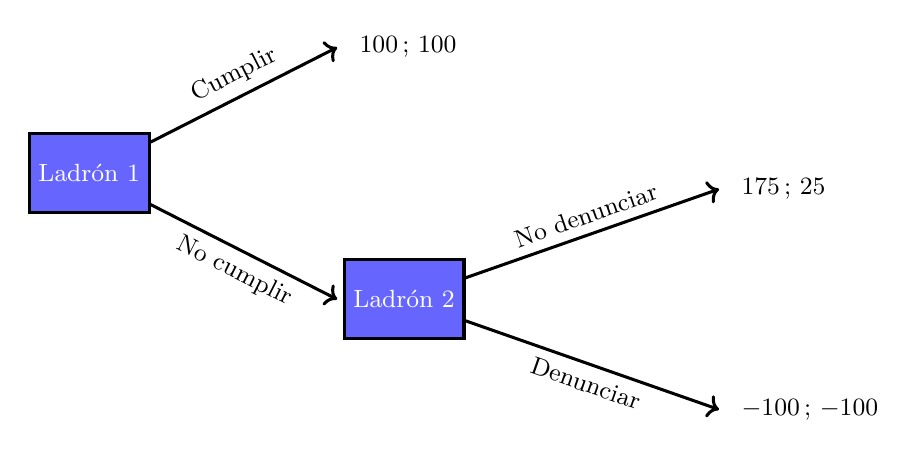
\begin{tikzpicture}[line width=1.1pt , every node/.style={font=\small}]

% Nodos (rectángulos azules)
\node[draw, fill=blue!60, text=white, minimum width=1.4cm, minimum height=1.0cm] (L1) at (0,0) {Ladrón 1};
\node[draw, fill=blue!60, text=white, minimum width=1.4cm, minimum height=1.0cm] (L2) at (4,-1.6) {Ladrón 2};

% Destinos (coordenadas de las hojas)
\coordinate (p11) at (3.15, 1.6); % 100 ; 100
\coordinate (p21) at ($(L2)+(4, 1.4)$);  % 175 ; 25
\coordinate (p22) at ($(L2)+(4,-1.4)$);  % -100 ; -100

% Ramas desde L1
\draw[->] (L1) -- (p11) node[midway, above, sloped]{Cumplir};
\draw[->] (L1) -- (3.15,-1.6)  node[midway, below, sloped]{No cumplir};

% Ramas desde L2
\draw[->] (L2) -- (p21) node[midway, above, sloped]{No denunciar};
\draw[->] (L2) -- (p22) node[midway, below, sloped]{Denunciar};

% Pagos (a la derecha de las puntas de flecha)
\node[anchor=west] at ($(p11)+(0.15,0)$) {$100\,;\,100$};
\node[anchor=west] at ($(p21)+(0.15,0)$) {$175\,;\,25$};
\node[anchor=west] at ($(p22)+(0.15,0)$) {$-100\,;\,-100$};

\end{tikzpicture}
\vspace{4mm}
Para resolver este problema, vamos a utilizar la inducción hacia atrás.
\end{frame}


\begin{frame}{El robo al Banco Rio}
    \begin{itemize}
        \item Lo primero que vamos a hacer es observar qué le conviene hacer al Ladrón 2 si el Ladrón 1 no cumple su promesa.
         \begin{itemize}
        \item Si el Ladrón 1 no cumple su promesa, al Ladrón 2 ¿le conviene aceptar o no aceptar? Como su pago es \$25 millones si acepta y -\$100 millones si no acepta, claramente
        le convendrá aceptar.
        \item Si el Ladrón 2 amenaza con denunciar al Ladrón 1, decimos que nos encontramos ante una "amenaza no creíble".
        \end{itemize}
        \item Dado que sabemos que al Ladrón 2 siempre le va a convenir aceptar, ¿qué le conviene al Ladrón 1?
       \begin{itemize}
        \item Si cumple, obtiene un pago de 100 y, si no cumple, de 175 (dado que el Ladrón 2 acepta)
        \end{itemize}
        \item El equilibrio de Nash es que el Ladrón 1 no cumple y el Ladrón 2 acepta.
        \begin{boxB}
            \centering \small
            Con inducción hacia atrás, recorremos ``hacia atrás'' el ``árbol'' hasta llegar
            al nodo inicial, identificando en cada nodo la estrategia óptima en
            anticipación del comportamiento que se espera hacia adelante.            
        \end{boxB}
    \end{itemize}
\end{frame}

\begin{frame}{Conclusión}
    \begin{itemize}
        \item Ciertos comportamientos y ciertas configuraciones pueden generar resultados que no sean los óptimos desde el punto de vista social.
        \item La teoría de juegos es una herramienta muy útil para entender y modelar comportamientos estratégicos.
        \item Además, es útil para pensar en los efectos de políticas públicas y en las expectativas que tienen los agentes.
    \end{itemize}
\end{frame}


\end{document}